\documentclass{beamer}

\usepackage{mathlist}

\usepackage[utf8]{inputenc}
\usetheme{Singapore}
\usepackage{xcolor}
\setbeamertemplate{footline}[frame number]

\newtheorem{defi}{Definition}
\newtheorem{theo}{Theorem}
\newtheorem{coro}{Corollary}
\newtheorem{lem}{Lemma}

\usepackage{epic,eepic}
\usepackage{pstricks, pst-tree}

\usepackage{times}

\usepackage{ulem}

\usepackage{listings}
%\topmargin=-0.6in
\lstloadlanguages{C++}
\lstset{language=C++}
%%}

\setbeamercovered{dynamic}

\def\bxi{\boldsymbol\xi}
\def\bepsilon{\boldsymbol\epsilon}
\def\bomega{\boldsymbol\omega}
\def\aff{\operatorname{aff}}
\def\cQ{\mathcal{Q}}

\newcommand{\tim}[1]{\;\; \mbox{#1} \;\;}

\title[SAA]{Stochastic Optimization\\Sample Average Approximation}

\author[Fabian Bastin]{Fabian Bastin \\ \url{bastin@iro.umontreal.ca} \\ Université de Montréal -- CIRRELT -- IVADO -- Fin-ML}

\date{}

\setbeamertemplate{footline}[frame number]

\begin{document}

\frame{\titlepage}

\begin{frame}
\frametitle{Framework}

Consider the stochastic program
\[
{\red \min_{z \in S} g(z) = E_P \left[ G(z, \bxi) \right]},
\]
\vspace{-0.5cm}
\begin{itemize}
\item 
$S \subset \rit^m$, compact;
\item
$\bxi$ is a random vector defined on $( \Xi, \mathcal{F}, P )$ and taking values in $( \rit^k, \mathcal{B}^k )$ %($\mathcal{B}^k$ is the Borel measure).;
\item
$G: \rit^m \times \rit^k \rightarrow \rit$;
\item
$E_P[\cdot]$ is the expectation with respect to $P$.
\end{itemize}

We assume that for each $z \in S$, the expected value function $g(z)$ is well defined, i.e. the function $G(z,\cdot)$ is $\mathcal{F}$-measurable and $P$-integrable.

\mbox{}

For simplicity, we assume for now that {\blue $S$ is deterministic}.

\end{frame}

\begin{frame}
\frametitle{Framework (cont'd)}

If the cumulative distribution function of $\bxi$ is continuous or discrete with a large number of possible realizations, $g(z)$ is usually very difficult to evaluate.

\mbox{}

We have to use some approximations as the Monte Carlo methods: the original problem is replaced by successive approximations obtained by drawing $\xi_1,\ldots{}, \xi_N$.
The approximation for a sample of size $N$ is
\[
{\red \min_{z \in S} \hat{g}_N(z) = \frac{1}{N} \sum_{i = 1}^N
  G(z, \xi_i)}.
\]
We sometimes refer to the original program as the {\blue true program}, or {\blue expected value program}, and the approximate program as the {\blue sample average approximation (SAA)}.

\end{frame}

\begin{frame}
\frametitle{Two-stage stochastic programming}

This framework include the two-stage programs that we have analyzed, as
\begin{align*}
\min_x\ & c^Tx + E[\cQ(x)] \\
\mbox{s.t. } & Ax = b,\ x \geq 0
\end{align*}
is equivalent to
$$
\min_{x \in S} E[c^Tx + \cQ(x)],
$$
where $S = \{ x \,|\, Ax = b, x \geq 0 \}$

\end{frame}

\begin{frame}
\frametitle{First-order convergence}

What happens when $N \rightarrow \infty$?

\mbox{}

Let {\red $z_N^*$ be a first-order critical point} for the approximate problem, i.e. the KKT conditions are satisfied at $z_N^*$.

\mbox{}

$(\xi_1,\ldots,\xi_N)$ can be seen as the finite truncature of an infinite sequence $\overline{\xi} := \lbrace \xi_k \rbrace_{k =   1}^{\infty}$.

\mbox{}

Solution for a sample size $N$: $z_N^*(\xi_1,\ldots,\xi_N)$, or $z_N^*\left(\overline{\xi}\right)$.

\mbox{}

As $S$ is a compact set, the sequence of SAA solutions has a non-empty set of (finite) limit points.

\mbox{}

{\blue Under which conditions such a limit point is a first-order critical point for the true problem?}

\end{frame}

\begin{frame}
\frametitle{Formalization}

%As the set of limit points depends on the realizations sequence $\overline{\xi}$, we introduce an adapted probability space over which we can define random variables whose realization are such (infinite) sequences

%\mbox{}

Consider the stochastic process
\[
\overline{\bxi} = \lbrace \bxi_k \rbrace_{k = 1}^{\infty},
\]
later called the sampling process, where the random vectors $\bxi_k$, $k = 1,\ldots, \infty$, are assumed to be independent and identically distributed (i.i.d.).

\end{frame}

\begin{frame}
\frametitle{Probability space of infinite dimension}

From the i.i.d. property and the Kolmogorov consistency theorem (see for instance Parthasarathy, {\sl Probability Measures on Metric   Spaces}, Academic Press, 1967, Chapiter~V, Theorem 5.1), we can build the probability space of infinite dimension
\[
\left( \Xi_{\Pi}, \mathcal{F}_{\Pi}, P_{\Pi} \right),
\]
where the measure $P_{\Pi}$ has the property that for any non-zero natural $j$,
\[
P_{\Pi}[B] = \prod_{i = 1}^j P[B_i],
\]
for any set $B = \prod_{i=1}^j B_i \times \prod_{i=j+1}^{\infty} \Xi$, with $B_i \in \mathcal{F}$, $i =
1,\ldots,j$.

\end{frame}

\begin{frame}
\frametitle{Probability space of infinite dimension (cont'd)}

In other terms, the marginal measures defined on $\prod_{i = 1}^j (\Xi, \mathcal{F})$, with finite $j$, $j \geq 1$, correspond to the product measures $\prod_{i = 1}^j P$, as expected.

\mbox{}

We therefore can see $\overline{\bxi}$ as a random variable on $\left( \Xi_{\Pi}, \mathcal{F}_{\Pi}, P_{\Pi} \right)$, whose realizations are processes formed by the successive draws $\xi_k$, $k = 1,\ldots,\infty$, i.e. 
$\overline{\xi} = \lbrace \xi_k \rbrace_{k = 1}^{\infty}$.

\mbox{}

{\blue Notations:}
\begin{itemize}
\item $\overset{a.s.}{\longrightarrow}$: almost sure;
\item $\overset{p}{\rightarrow}$: convergence in probability;
\item $\Rightarrow$: convergence in distribution.
\end{itemize}

\end{frame}

\begin{frame}
\frametitle{Probability notions: types of convergence}

\begin{defi}[Almost sure convergence (or with probability one)]
A sequence of random variables $\lbrace \bxi_n \rbrace_{n = 1}^{+\infty}$ converges almost surely to a random variable $\bxi$ if
\[
P_{\bxi} [ \lbrace \omega |\, \bxi_n(\omega) \rightarrow \bxi(\omega)
\text{ as } n \rightarrow \infty \rbrace ] = 1.
\]
\end{defi}
% définition équivalente: chap 18.

\mbox{}

A weaker convergence mode is defined below.

\begin{defi}[Convergence in probability]
The sequence of random variables $\lbrace \bxi_n \rbrace_{n =
  1}^{+\infty}$ converges in probability to the random variable $\bxi$ if, for all $\epsilon > 0$,
\[
\lim_{n \rightarrow \infty} P_{\bxi} [ \lbrace \omega \,|\, |
\bxi_n(\omega) - \bxi(\omega) | \geq \epsilon \rbrace ] = 0.
\]
\end{defi}

\end{frame}

\begin{frame}
\frametitle{Probability notions: types of convergence (cont'd)}

Almost sure convergence implies converge in probability; the converse is not true.

\begin{defi}[Convergence in distribution]
Given a sequence of random variables $\lbrace \bxi_n \rbrace_{n=1}^{\infty}$ and a random variable $\bxi$, $\bxi_n$ converges in distribution to $\bxi$ if $\bxi_n$ if
$$
\lim_{n \rightarrow \infty} F_n(x) \rightarrow F(x)
$$
for each $x \in %C$, where $C \subseteq
\rit$ %is the set of points
where $F$ is continuous. $F_n$ and $F$ are the distribution functions of $\bxi_n$ and $\bxi$, respectively.

\mbox{}

We will also note $\bxi_n \Rightarrow \bxi$.
\end{defi}

\mbox{}

%To say that a sequence of random variables converges in distribution only means that the limit random variable has a given distribution.
If both $\bxi$ and $\boldsymbol{\zeta}$ follow the distribution specified by $F$, then $\bxi_n \Rightarrow \bxi$ and $\bxi_n \Rightarrow \boldsymbol{\zeta}$ are equivalent statements.

\end{frame}

\begin{frame}
\frametitle{Notations}

We will assume that the expressions  \textsl{\blue almost everywhere} (a.e.) and \textsl{\blue almost surely} (a.s.) refer to the infinite dimension space  $\left( \Xi_{\Pi}, \mathcal{F}_{\Pi}, P_{\Pi} \right)$, allowing to %explicitly
consider sets of realizations %whose elements have
of the form $\{\xi_n\}_{n=1}^{\infty}$.

\mbox{}

%(In other words, the related results hold for almost every sampling process.)

%\mbox{}

%A reference to another probability space will be denoted by prefixing the terms \textsl{almost surely} and \textsl{almost surely} by the measure defined on this probability space, and the expression \textsl{almost all sampling process} will be prefixed by the probability measure associated to the probability space of each process element.

\end{frame}

\begin{frame}
\frametitle{Assumptions}

\noindent
\textbf{A.0}
The random draws $\lbrace \xi_k \rbrace_{k= 1}^{\infty}$ are i.i.d.

\mbox{}

\noindent
\textbf{A.1}
For $P$-almost all $\xi$, the function $G(\cdot, \xi)$ is continuously differentiable on $S$.

\mbox{}

\noindent
\textbf{A.2}
The family $G(z, \xi)$, $z \in S$, is dominated by a $P$-integrable function $K(\xi)$, i.e. $E_P[K]$ is finite and $| G(z, \xi) | \leq K(\xi)$ for all $z \in S$ and $P$-almost each $\xi$.

\end{frame}

\begin{frame}
\frametitle{Assumptions: discussion}

\textbf{A.1} obviously implies that $G(\cdot, \xi)$ is $P$-almost surely continuous.

\mbox{}

This last property and \textbf{A.2}, are typical assumptions in stochastic programming (see for instance Rubinstein and Shapiro, {\sl Discrete Event Systems}, John Wiley \& Sons, 1993).

\mbox{}

The stronger form \textbf{A.1} is justified by our interest in the first-order optimality conditions.%, which are expressed in term of the gradient of the objective.

\end{frame}

\begin{frame}
\frametitle{Uniform law of large numbers}

\textbf{A.0}--\textbf{A.2} together imply that there exists an {\blue uniform law of large numbers (ULLN)} on $S$, for the approximation $\hat{g}_n(z)$ of $g(z)$:% that is
\[
\sup_{z \in S} \left| \hat{g}_n(z) - g(z) \right|
\overset{a.s.}{\longrightarrow} 0
\quad \mbox{as} \; n \rightarrow \infty.
\]
%The ULLN property corresponds to the stochastic version of the uniform
%convergence of a sequence of functions, and \textbf{A.0}--\textbf{A.2}
This also implies that $g(z)$ is continuous on $S$.

\mbox{}

\begin{footnotesize}
Reminder: the law of large numbers concerns the convergence of an empirical mean to the expectation of the random variable under consideration.
The convergence can be in probability (weak law) or almost surely (strong law).
\end{footnotesize}

\mbox{}

Our motivation to study the first-order conditions leads us to introduce an additional assumption on the gradient.

\mbox{}

\noindent
\textbf{A.3}
Each gradient component $\frac{\partial}{\partial [z]_l} G(z, \xi)$ ($l = 1,\ldots,m$), $z \in S$, is dominated by a $P$-integrable function.

\end{frame}

\begin{frame}
\frametitle{Consequences}

\textbf{A.3} implies that the expected value function $g(z)$ is continuously differentiable on $S$, and
\[
\nabla_z g(z) = E_P\left[ \nabla_z G(z, \bxi) \right].
\]

\mbox{}

Thus, $\nabla \hat{g}_n(z^*)$ is an unbiased estimator of $\nabla g( z^*)$.

\mbox{}

The {\blue first-order convergence} can be derived from the stochastic variational inequalities, as presented in A. Shapiro, {\sl Monte Carlo sampling methods},
in A.~Shapiro and A.~Ruszczy\'nski, editors, {\sl Stochastic Programming}, volume~10 of {\sl Handbooks in Operations Research and Management Science}, pages 353--425. Elsevier, 2003.

\end{frame}

\begin{frame}
\frametitle{Stochastic variational inequalities}

Consider a mapping $\Phi: \rit^m \times \rit^k \rightarrow \rit^m$ and a multi-function $\Gamma: \rit^m \rightrightarrows  \rit^m$, and suppose that $\phi(z) := E_{P}[\Phi(z, \bxi)]$ is well defined.
We denote
\[
\phi(z) \in \Gamma(z)
\]
as the true {\blue generalized equation}, or in expected value.
$z^* \in \rit^m$ is a solution of the generalized equation if $\phi(z^*) \in \Gamma(z^*)$.

\mbox{}

If $\lbrace \xi_1,\ldots,\xi_n \rbrace$ is a random sample, we denote
\[
\hat{\phi}_n(z) \in \Gamma(z)
\]
as the generalized SAA equation, where $\hat{\phi}_n(z) = n^{-1}\sum_{i=1}^n \Phi(z,\xi_i)$.
We denote by $S^*$ and $S^*_n$ the set of (all) solutions of the generalized equations in expected value and from the SAA, respectively.

\end{frame}

\begin{frame}
\frametitle{First-order convergence}

Denote by $d(x,A) := \inf_{x' \in A} \| x - x' \|$, the distance from $x \in \rit^m$ to $A$, and $D(A,B) := \sup_{x \in A} D(x, B)$, the deviation of the set $A$ from the set $B$.
We have the following result (Shapiro, 2003).
\begin{theo}[Generalized equations]
Let $\mathcal{S}$ be a compact subset of $\rit^m$ such that $S^* \subseteq \mathcal{S}$.
Assume that
\begin{enumerate}[(a)]
\item
the multi-function $\Gamma(z)$ is closed, i.e. if $z_k \rightarrow z$, $y_k \in \Gamma(z_k)$ and $y_k \rightarrow y$, then $y \in \Gamma(z)$,
\item
the mapping $\phi(z)$ is continuous on $\mathcal{S}$,
\item 
almost surely, $\emptyset \neq S^*_n \subseteq \mathcal{S}$ for $n$ large enough, and
%we have that
%\[
% P_{\Pi} [ \exists N_0 \tim{such that for all} N > N_0, S^*_N \tim{is
%    non-empty and} S^*_N \subset \mathcal{S}] = 1
%\] and
\item
$\hat{\phi}_n(z)$ converges to $\phi(z)$ almost surely uniformly of $\mathcal{S}$ as $n \rightarrow \infty$.
\end{enumerate}
Then $D(S^*_n, S^*) \rightarrow 0$ almost surely as $n \rightarrow \infty$.
\label{th:svi}
\end{theo}

\end{frame}

\begin{frame}
\frametitle{First-order optimality conditions}

We denote the feasible set of a mathematical program by $\mathcal{A}$.
We will suppose here that $\mathcal{A}$ is closed.

\mbox{}

{\red Necessary condition}: if $x^*$ is a local minimizer,
\[
-\nabla_x f(x^*) \in \mathcal{N}_{\mathcal{A}}(x^*),
\]
where $\mathcal{N}_{\mathcal{A}}(x^*)$ is the normal cone to $\mathcal{A}$ at $x^*$.

\mbox{}

{\blue Cone}

\mbox
 
A subset $C$ of a vectorial space $V$ is a (linear) {\red cone}
iff $\alpha x$ belongs to $C$ for any $x \in C$ and any strictly positive scalar $\alpha$.
It is pointed if $\alpha$ can be equal to zero.

\mbox{}

A {\red convex cone} is a cone closed under convex combinations, i.e. iff $\alpha x + \beta y \in C$, $\forall \alpha,\ \beta > 0$, with $\alpha + \beta = 1$.

\end{frame}


\begin{frame}
\frametitle{Tangent cone, normal cone: general framework}

We first say that a vector $w \in \rit^n$ is tangent to $\mathcal{A}$ at $x \in \mathcal{A}$ if for all sequences of vectors $\lbrace x_i \rbrace$ with $x_i \rightarrow x$, and $x_i \in \mathcal{A}$, and all sequences of positive scalars $t_i \downarrow 0$, there exists a sequence $w_i \rightarrow w$ such that $x_i + t_iw_i \in \mathcal{A}$ for all $i$.

\mbox{}

The {\red tangent cone $T_{\mathcal{A}}(x)$} is the collection of vectors tangent to ${\mathcal{A}}$ at $x$. \\
The {\red normal cone $N_{\mathcal{A}}(x)$} is the orthogonal complement, i.e.
\[
N_{\mathcal{A}}(x) = \lbrace v\ |\ v^Tw \leq 0,\ \forall w \in T_{\mathcal{A}}(x) \rbrace.
\]

\mbox{}

OK, but in practice???

\end{frame}

\begin{frame}
\frametitle{Tangent cone, normal cone (cont'd)}

If ${\mathcal{A}}$ is convex,
$
\mathcal{N}_{\mathcal{A}}(x) = \left\lbrace v\ |\ v^T(x-x_0) \geq 0,\ \forall x_0 \in
{\mathcal{A}} \right\rbrace.
$

\mbox{}

The condition becomes
$\nabla_x f(\hat{x})^T (x-\hat{x}) \geq 0$, $\forall x \in {\mathcal{A}}$.

\mbox{}

If $f$ is convex (i.e. we are in the convex programming framework), the condition is also sufficient.

\end{frame}

\begin{frame}
\frametitle{Deterministic and convex constraints}

Therefore, when $S$ is convex, we can rewrite the first-order criticality conditions at some point $z^*$ as the requirement that $-\nabla_z g(z^*)$ belongs to the normal cone to $S$ at $z^*$, denoted by $\mathcal{N}_{S}(z^*)$.

\mbox{}

If moreover $S$ is deterministic, the feasible sets are the same for the true and SAA problems.

\mbox{}

The previous theorem allows us to easily establish the first-order convergence.
Consider the choice $\Gamma(\cdot) = \mathcal{N}_S(\cdot)$; $\phi(z^*)$ belongs to $\Gamma(z^*)$ iff
\[
\langle \phi(z^*), u-z^*\rangle \leq 0,\ \forall u \in S.
\]

We design such variational inequalities as \textcolor{red}{stochastic variational inequalities}.

\end{frame}

\begin{frame}
\frametitle{Convergence}

The assumption (a) of the theorem always holds in this case.
Take $\Phi(z,\xi) = -\nabla_z G(z, \xi)$ and represent by $S^*$ and $S^*_n$ the set of first-order critical points of the true and SAA generalized equations, respectively.

\begin{itemize}
\item
The assumption (a) holds by definition of the normal cone.
\item
Then, under \textbf{A.0}--\textbf{A.3}, we have that $\phi(z) = -\nabla_z
g(z)$, and that $\phi(z)$ is a continuous random vector on $S$, giving assumption (b).
\item
Assumption (d) follows from the ULLN, while \textbf{A.1} and the compacity of $S$ ensure assumption (c) by setting $\mathcal{S} = S$. 
\end{itemize}

The previous theorem ensures therefore the first-order criticality at the limit as $n\rightarrow\infty$, almost surely.

\end{frame}

\begin{frame}
\frametitle{Remark}

The theorem establishes that $D(S_n^*, S^*) \rightarrow 0$ when $n \rightarrow \infty$, almost surely. However, we cannot write $D(S^*, S_n^*) \rightarrow 0$ when $n \rightarrow \infty$, almost surely.

\mbox{}

Consider for instance the optimization problem
$$
\min_{x \in S} |E[\xi]| x^2,
$$
where $S = [-a,a]$, $a > 0$. If $\xi \sim N(0, \sigma^2)$, $S^* = S$.
The SAA approximation is
$$
\min_{x \in S} \left|\frac{1}{n} \sum_{i=1}^n \xi_i\right| x^2,
$$
and almost surely, $S^*_n = \{ 0 \}$. Therefore, a.s. $\lim_{n \rightarrow \infty} S^*_n = \{ 0 \} \ne S^*$, and $D(S^*, \{0\}) = a$.

\end{frame}

\begin{frame}
\frametitle{Stochastic constraints}

Under stronger assumptions, it is also possible to prove the first-order convergence almost surely when $S$ is non-convex or non-deterministic.

\mbox{}

We now assume that the feasible set can be described by equality and inequality constraints.
The original problem now becomes
\begin{align*}
\min_{z \in V}\ & g(z) = E_P[G(z, \boldsymbol{\xi})],\\
\text{such that } & c_j(z) \geq 0,\ j = 1,\ldots,k,\\
& c_j(z) = 0,\ j = k+1,\ldots, M,
\end{align*}
where $V$ is a compact subset of $\rit^m$.

\end{frame}

\begin{frame}
\frametitle{Stochastic constraints (cont'd)}

The corresponding SAA problem is defined as
\begin{align*}
\min_{z \in V}\ & \hat{g}_n(z),\\
\text{such that } & \hat{c}_{jn}(z) \geq 0,\ j = 1,\ldots,k,\\
& \hat{c}_{jn}(z) = 0,\ j = k+1,\ldots, M.
\end{align*}

\mbox{}

Here, for each $j = 1,\ldots,M$, $\lbrace \hat{c}_{jn}(\cdot) \rbrace$ is a sequence of (random) functions converging asymptotically to the corresponding function $c_j(\cdot)$ as $n \rightarrow \infty$.

\mbox{}

We assume that the functions $c_j(\cdot)$ can be represented in form of expectations:
\[
c_j(z) = E_P[H_j(z,\boldsymbol{\xi})],\ j = 1,\ldots,M.
\]

\end{frame}

\begin{frame}
\frametitle{Stochastic constraints (cont'd)}

These functions can then be approximated by corresponding sample average approximations:
\[
\hat{c}_{jn}(z) = \frac{1}{n} \sum_{i = 1}^n H_j(z,\xi_i).
\]

\mbox{}

For simplicity, we consider the more general parametric mathematical problem
\begin{align*}
\min_{z \in V}\ & \hat{g}(z, \bepsilon),\\
\text{such that } & \hat{c}_j(z, \bepsilon) \geq 0,\ j
= 1,\ldots,k,\\
& \hat{c}_j(z, \bepsilon) = 0,\ j = k+1,\ldots, M,
\end{align*}
where $\bepsilon$ is a parametric random vector giving the perturbations of the approximated program, and $g(\cdot)$, $\hat{g}(\cdot, \bepsilon)$, $c_j(\cdot)$, $\hat{c}_j(\cdot, \bepsilon)$ are assumed to be of class $C^2$ with respect to $z$.

\end{frame}

\begin{frame}
\frametitle{Random perturbations}

We assume that the perturbation has the form
\[
\bepsilon = \bepsilon(z,\overline{\xi}) =
\begin{pmatrix} \bepsilon_g,\
\bepsilon_{c_1},\ 
\ldots,\ 
\bepsilon_{c_M},\ 
\bepsilon^T_{\nabla g},\ 
\bepsilon^T_{\nabla c_1},\ 
\ldots,\ 
\bepsilon^T_{\nabla c_M}
\end{pmatrix}^T,
\]
where each component is function from $\rit^m \times \prod_{i = 1}^{\infty} \rit^k$ to $\rit$ or $\rit^m$, and
\[
\begin{aligned}
\hat{g} (z, \boldsymbol{\epsilon}) = g(z) + \boldsymbol{\epsilon}_g,\ &
\nabla_z \hat{g} (z, \boldsymbol{\epsilon}) = \nabla_z g(z) +
\boldsymbol{\epsilon}_{\nabla g}, \\
\hat{c}_j (z, \boldsymbol{\epsilon}) = c_j(z) +
\boldsymbol{\epsilon}_{c_j},\ &
\nabla_z \hat{c}_j (z, \boldsymbol{\epsilon}) = \nabla_z c_j(z) +
\boldsymbol{\epsilon}_{\nabla c_j},\ j = 1,\ldots, M.
\end{aligned}
\]

\mbox{}

We also define $\epsilon_n (z, \overline{\xi} )$ as
\[
\epsilon_n(z, \overline{\xi}) = \begin{pmatrix} \hat{g}_n(z)-g(z) \\
\hat{c}_{jn}(z)-c_j(z),\ j=1,\ldots,M\\
\nabla_z \hat{g}_n(z) -
\nabla_z g(z)\\
\nabla_z \hat{c}_{jn}(z)- \nabla_z c_j(z),\ j=1,\ldots,M \end{pmatrix},
\]

\end{frame}

\begin{frame}
\frametitle{Random perturbations (cont'd)}

We denote the corresponding random vector by $\boldsymbol{\epsilon}_n (z, \overline{\bxi} )$, and we will assume the ULLN holds for the objective and 
the constraints, as well as for their corresponding derivatives.

\mbox{}

We finally assume that the feasible set for the original and approximated problems are non-empty.
The Lagrangians of the true and approximated problems are respectively
\[
\mathcal{L}(z, \lambda) = g(z) - \sum_{j = 1}^M [\lambda]_j c_j(z)
\]
and
\[
L(z, \lambda, \boldsymbol{\epsilon}) = \hat{g}(z,
\boldsymbol{\epsilon}) - \sum_{j = 1}^M [\lambda]_j \hat{c}_j(z,
\boldsymbol{\epsilon}).
\]

\end{frame}

\begin{frame}
\frametitle{KKT conditions}

Let $z^*(\bepsilon)$ be a first-order critical point of the approximated program, and assume that $z^*(\bepsilon)$ belongs to the interior of $V$, that we denote by $\overset{o}{V}$.

\mbox{}

There exist Lagrange multipliers $\lambda^*(\boldsymbol{\epsilon})$ such that $(z^*(\boldsymbol{\epsilon}), \lambda^*(\boldsymbol{\epsilon}))$ satisfies the KKT conditions; in other terms $(z^*(\boldsymbol{\epsilon}), \lambda^*(\boldsymbol{\epsilon}))$ is solution to the system
\[
\begin{aligned}
\nabla_z L(z, \lambda, \boldsymbol{\epsilon}) = 0,\\
[\lambda]_j\hat{c}_j(z, \boldsymbol{\epsilon}) = 0, &\quad j = 1,\ldots,M,\\
\hat{c}_j(z, \boldsymbol{\epsilon}) = 0, &\quad j = k+1,\ldots,M,\\
\hat{c}_j(z, \boldsymbol{\epsilon}) \geq 0, &\quad j = 1,\ldots,k,\\
[\lambda]_j(\boldsymbol{\epsilon}) \geq 0, &\quad j = 1,\ldots,k.
\end{aligned}
\]

\end{frame}

\begin{frame}
\frametitle{Solution characteristics}

Consider now the specific sampling process $\overline{\xi}$.
In order to emphasize the dependency of the first-order critical points to the sampling process, we denote $z_n^*(\overline{\xi})$ for $z^*(\epsilon_n)$ and $\lambda_n^*(\overline{\xi})$ for $\lambda^*(\epsilon_n)$.
%As before, since $V$ is compact, $z^*_N(\overline{\xi})$ has some limit
%point $z^*(\overline{\xi})$ as $N \rightarrow \infty$.

\mbox{}

Let $\mathcal{Z}\left(\lbrace z^*_n(\overline{\xi})\rbrace\right)$ the set of accumulation points of the sequence $\lbrace z_n^*(\overline{\xi}) \rbrace_{n = 1}^{\infty}$.
%\[
%\mathcal{Z} : \prod_{i=1}^{\infty} \rit^m_i \rightrightarrows \rit^m,
%\]
%be the multifunction associating to a sequence of real vectors its set of
%accumulation points.
The compacity of $V$ implies that for each $\overline{\xi}$, %the set
$\mathcal{Z}\left(\lbrace z^*_n(\overline{\xi})\rbrace\right)$ is non-empty.

\mbox{}

We can now prove the first-order convergence for the general case.

\end{frame}

\begin{frame}
\frametitle{First-order convergence}

\begin{small}

\begin{theo}
\label{th:fod_first}
Assume that for almost every $\overline \zeta$ in $(\Xi_{\Pi}, \mathcal{F}_{\Pi}, P_{\Pi})$, $\epsilon_n(z, \overline{\zeta}) \rightarrow 0$ uniformly on the compact set $V$, as $n \rightarrow \infty$, and let $\overline \xi$ in $(\Xi_{\Pi}, \mathcal{F}_{\Pi}, P_{\Pi})$ satisfying the assumption of uniform convergence.

If $z^* \in \mathcal{Z}\left(\lbrace z^*_n(\overline{\xi})\rbrace\right)$ belongs to $\overset{o}{V}$, and a sub-sequence $\lbrace z^*_{\ell}(\overline{\xi}) \rbrace_{\ell = 1}^{\infty} \subseteq \lbrace z^*_n (\overline{\xi}) \rbrace_{n = 1}^{\infty}$ converging to $z^*$ is associated to a sequence of Lagrange multipliers $\lbrace \lambda^*_{\ell} (\overline{\xi}) \rbrace_{\ell = 1}^{\infty}$ with a least one limit point, then $z^*$ is a first-order critical point of the true problem.
\end{theo}

\begin{proof}
From our assumptions, the sequence $\left\lbrace (z^*_{\ell}(\overline{\xi}), \lambda^*_{\ell}(\overline{\xi}) \right\rbrace$, $\ell=1,\ldots,\infty$, has a limit point $( z^*, \lambda^* )$.
The uniform convergence property implied that $( z^*, \lambda^* )$ satisfies the KKT conditions of the true problem, so that $z^* (\in \overset{o}{V})$ is first-order critical point of the original problem.
\end{proof}

\end{small}

\end{frame}

\begin{frame}
\frametitle{On the Lagrange multipliers}

The assumption of Lagrange multipliers convergence always holds if the Lagrange multipliers are bounded.
This stronger assumption allows us to use the convergence results on the variational inequalities in order to prove the first-order criticality of limit points (Shapiro, 2003).
%conditions of Theorem~\ref{th:fod_first} is first-order critical,

\mbox{}

Let $\mu := (z,\lambda) \in \rit^{m+M}$ and $\mathcal{K} := \rit^m
\times \rit^k_+ \times \rit^{M-k} \subset \rit^{m+M}$.
Define
\begin{align*}
\phi(\mu) &= \left( \nabla_z \mathcal{L}(z, \lambda), c_{k+1}(z),
\ldots, c_M(z) \right),\\
\hat{\phi}_n(\mu) &= \left( \nabla_z L(z, \lambda, \bepsilon_n),
\hat{c}_{k+1}(z, \bepsilon_n), \ldots, \hat{c}_{M}(z,
\bepsilon_n)\right).
\end{align*}
The generalized equation $\phi(\mu) \in \mathcal{N}_{\mathcal{K}}(\mu)$ then represents the KKT optimality conditions for the original optimization problem, $S^* \subseteq \overset{o}{V}$, and the theorem on generalized equations then implies first-order criticality almost surely, with $\Gamma(\mu) := \mathcal{N}_{\mathcal{K}}(\mu)$.

\end{frame}

\begin{frame}
\frametitle{On the Lagrange multipliers (cont'd)}

Assumptions $(a)$ and $(d)$ of the theorem on generalized equations are sufficient as $\bepsilon \rightarrow 0$ almost surely, and assumption $(c)$ holds as feasible set for original and approximate problems are non-empty.

\mbox{}

Trickier: second-order.

\end{frame}

\begin{frame}
\frametitle{Second-order convergence}

If we strengthen our assumptions, we can also show that, almost surely, there exists limit points in $\mathcal{Z}\left(\lbrace z^*_n(\overline{\bxi})\rbrace\right)$ that are local minimizers.

\mbox{}

We first consider the case where $S$ is deterministic and assume that, for a given sampling process $\overline{\xi}$, $z_n^*(\overline{\xi})$ is a local minimizer of $\hat{g}_n(z)$ over $S$.
In other terms,
\[
\exists\, \delta_n(\overline{\xi}) \text{ t.q. } \forall z \in
B \left( z_n^*(\overline{\xi}), \delta_n(\overline{\xi}) \right) \cap
S,\ \hat{g}_n \left( z_n^*(\overline{\xi}) \right) \leq \hat{g}_n(z).
\]
%where $B(x,d)$ is an open ball centered at $x$ and with radius $d$.

\end{frame}

\begin{frame}
\frametitle{A counter-example}

Consider the problem
\begin{equation}\label{eq:ex_true}
\min_{z \in [-1, 1]} z^3 - \frac{z}{2}E_P[\bxi],
\end{equation}
where $\Xi = \lbrace -1, 1\rbrace$ and $P[\xi = -1] = P[\xi = 1] = 0.5$, so $E_P[\bxi] = 0$, and \eqref{eq:ex_true} has one local minimizer only, that is also global, at $z^* = -1$.
The SAA problem is then
\begin{equation}\label{eq:ex_approx}
\min_{z \in [-1, 1]} z^3 - \frac{z}{2n}\sum_{i = 1}^n \xi_i.
\end{equation}
Problem \eqref{eq:ex_approx} has two (isolated) local minimizers
\[
\left\lbrace -1, \sqrt{\frac{\sum_{i=1}^n \xi_i}{6n}}\right\rbrace,
\]
when $\sum_{i=1}^n \xi_i > 0$.
As $n \rightarrow \infty$, we have $P\left[\sum_{i=1}^n \xi_i > 0\right] \rightarrow 0.5$, but from the ULLN, $\frac{1}{6n}\sum_{i=1}^n \xi_i \rightarrow \frac{1}{6}E_P[\bxi] = 0$ a.s.
% However zero is a saddle point of the true
%problem \eqref{eq:ex_true}, not a minimizer, even locally, and the
%distance to $S^* = \lbrace -1 \rbrace$ is then equal to 1. Note that
%in this example the ULLN holds for the objective function as well as
%for all its derivatives.

\end{frame}

\begin{frame}
\frametitle{Rigidity assumption}

(Bastin, Cirillo, and Toint, 2006, Pasupathy, 2010)


In order to show that $z^* \in \mathcal{Z}\left(\lbrace z^*_n(\overline{\xi})\rbrace\right)$ is a local minimizer of $g(\cdot)$ over $S$, 
we have to show that for some subsequence $\lbrace z^*_{\ell} (\overline{\xi}) \rbrace_{\ell = 1}^{\infty} \subseteq \lbrace z^*_{n} (\overline{\xi}) \rbrace_{n = 1}^{\infty}$ converging to $z^*$, the neighborhood where $z_{\ell}^*(\overline{\xi})$ is a local minimizer do not reduce to a singleton as $\ell \rightarrow \infty$.

\mbox{}

We express this requirement with the technical assumption.

\noindent
\textbf{A.4}
There exists some subsequence $\left\lbrace z^*_{\ell} (\overline{\xi}) \right\rbrace_{\ell = 1}^{\infty}$ converging to some $z^*$, with $\left\lbrace z^*_{\ell} (\overline{\xi}) \right\rbrace_{\ell = 1}^{\infty} \subseteq \left\lbrace z^*_{N} (\overline{\xi}) \right\rbrace_{N = 1}^{\infty}$, and some constants $\delta_{z^*\overline{\xi}} >0$ and $\ell_{z^* \overline{\xi}} > 0$ such that for all $\ell \geq \ell_{ z^* \overline{\xi}}$,
\[
\forall z \in B\left( z_{\ell}^*(\overline{\xi}), \delta_{z^*
  \overline{\xi}} \right) \cap S, \  \hat{g}_{\ell} \left(
  z_{\ell}^*(\overline{\xi}) \right) \leq \hat{g}_{\ell}(z).
\]


\end{frame}

\begin{frame}
\frametitle{Basic theorem}

\begin{theo}
\label{th:basic_second_order}
Assume that \textbf{A.0}--\textbf{A.3} hold.
Then, for almost every sampling process $\overline{\xi}$,
$\left \lbrace z^* \in \mathcal{Z}\left(\lbrace
    z^*_N(\overline{\xi})\rbrace\right) \text{ satisfying
    \textbf{A.4}} \right \rbrace$ is a set of local minimizers of $g(\cdot)$ over $S$.
\end{theo}

\begin{proof}
Voir Bastin, Cirillo, and Toint, {\sl Convergence theory for
  nonconvex stochastic programming with an application to mixed logit},
  Mathematical Programming, 108(2--3):207--234 (2006).
\end{proof}

\end{frame}

\begin{frame}
\frametitle{Stochastic constraints}

Assumption~\textbf{A.4} is somewhat artificial and it is therefore more interesting  to look for more elegant conditions.

\mbox{}

At the difference of classical sensitivity analysis, we focus here on conditions under which a limit point of a sequence of approximate solutions is a solution of the true problem.

\mbox{}

As previously, we consider the case where the feasible set is described by a set of equality and inequality constraints, and we assume that $\bepsilon_n$ converges to 0 almost surely, uniformly on $V$.

\end{frame}

\begin{frame}
\frametitle{Lagrange multipliers convergence}

Consider a particular sampling process $\overline{\xi}$ in $(\Xi_{\Pi}, \mathcal{F}_{\Pi}, P_{\Pi})$, and $z^*
\in \mathcal{Z}\left(\lbrace z^*_n(\overline{\xi})\rbrace\right)$.
Under some conditions, if the subsequence $\lbrace z_{\ell}^* \rbrace_{\ell =  1}^{\infty}$ converges to $z^*$, the sequence of associated Lagrange multipliers vectors $\lbrace \lambda_{\ell}^* \rbrace$ also converges to some Lagrange multipliers vector $\lambda^*$ associated to $z^*$ for the true problem.

\mbox{}

\begin{lem}
Consider a particular sampling process
$\overline{\xi}$ in $(\Xi_{\Pi}, \mathcal{F}_{\Pi}, P_{\Pi})$ such that
$\epsilon_n \left( z, \overline{\xi} \right) \rightarrow 0$
uniformly on $V$ as $n \rightarrow \infty$.
If $z^* \in \mathcal{Z} \left(\lbrace
z^*_n(\overline{\xi})\rbrace\right) \cap \overset{o}{V}$, $\lbrace
z_{\ell}^* \rbrace_{\ell =  1}^{\infty} \subseteq \lbrace z_n^*
\rbrace_{n =  1}^{\infty} \cap \overset{o}{V}$ converges to $z^*$,
and there exists some unique Lagrange multipliers vector associated to $z^*$ satisfying the KKT conditions, then $\lambda^*_{\ell}(\overline{\xi})$ converges to $\lambda^*$ as $\ell \rightarrow \infty$.
\end{lem}

\end{frame}

\begin{frame}
\frametitle{Lagrange multipliers convergence (cont'd)}

\begin{proof}
From the unicity of $\lambda^*$, the Mangasarian-Fromowitz constraint qualification (MFCQ) holds at $z^*$, and therefore in a neighborhood of $z^*$.
A consequence is that the Lagrange multipliers are uniformly bounded for $\epsilon$ close to zero.
It is therefore sufficient to show that every limit point of the sequence $\lbrace \lambda^*_{\ell}(\overline{\xi}) \rbrace$, $\ell = 1,\ldots,\infty$, is equal to $\lambda^*$.

\mbox{}

Let $\lambda'$ be such a limit point.
By continuity, $(z^*, \lambda' )$ satisfies the KKT conditions, so $\lambda'$ is equal to $\lambda^*$.
\end{proof}

\mbox{}

The unicity of $\lambda^*$ can be ensured with some appropriate constraints qualification condition, as the  linear independence constraint qualification (LICQ).

\end{frame}

\begin{frame}
\frametitle{On the LICQ}

This constraints qualification will be especially useful for our discusssion.

\mbox{}

Consider the original program.
Recall that the active set $\mathcal{A}(z)$ at any feasible point $z$ is the union of the index set of equality constraints and active inequality constraints:
\[
\mathcal{A}(z) = \lbrace i \in \lbrace 1,\ldots,k \rbrace \, | \,
c_i(z) = 0 \rbrace \cup \lbrace k+1,\ldots,M \rbrace.
\]

\begin{defi}
Given the point $z^*$ and the active set $\mathcal{A}(z^*)$, we say that the LICQ holds at $z^*$ if the set of active constraints gradients $\lbrace \nabla c_j(z^*),\ j \in \mathcal{A}(z^*) \rbrace$ is linearly independent.
\end{defi}

\end{frame}

\begin{frame}
\frametitle{Strict complementarity}

Another useful concept for our needs is the strict complementarity condition.

\begin{defi}
Given $z^*$ and a vector $\lambda^*$ satisfying the KKT conditions, we say that the strict complementarity condition holds if exactly one of $[\lambda]_j^*$ and $c_j(z^*)$ is null for every index $j=1,\ldots,k$, i.e. we have that $[\lambda]_j^* > 0$ for each $j \in \lbrace 1,\ldots,k \rbrace \cap \mathcal{A}(z^*)$.
\end{defi}

\mbox{}

Consider again a particular sampling process $\overline{\xi}$ dans $(\Xi_{\Pi}, \mathcal{F}_{\Pi}, P_{\Pi})$, such that $\epsilon_n (z, \overline{\xi} ) \rightarrow 0$ as $n \rightarrow \infty$. 
If the assumptions of the above lemma hold for some subsequence $\lbrace z_{\ell}^* \rbrace_{\ell = 1}^{\infty} \rightarrow z^*$, the gradient of the Lagrangian $\nabla L\left( z^*_{\ell} ( \overline{\xi} ), \lambda_{\ell}^* ( \overline{\xi} ) \right)$ converges to $\nabla \mathcal{L} ( z^*, \lambda^* )$, as $\ell$ tends to infinity, with $\lambda_{\ell}^*(\overline{\xi}) \rightarrow \lambda^*$.

\end{frame}

\begin{frame}
\frametitle{Strict complementarity (cont'd)}

Assume that the strict complementarity condition holds at $z^*$ for the approximate problem.
Then, for $\ell$ large enough,
$$
[\lambda^*_{\ell}]_j(\overline{\xi}) > 0,\, \forall j \in \lbrace 1,\ldots,k \rbrace \cap \mathcal{A} ( z^* ) .
$$
Thus the corresponding constraints are active at $z^*_{\ell}(\overline{\xi})$.

\mbox{}

Moreover, as $\epsilon_n (z, \overline{\xi} ) \rightarrow 0$,
$\hat{c}_j \left( z^*_{\ell}(\overline{\xi}),
\epsilon_{\ell}(z^*_{\ell}(\overline{\xi}),\overline{\xi}) \right) \rightarrow
c_j ( z^* )$ and, for $\ell$ large enough,
%(which is true for almost every  $\overline{\xi}$)
$\mathcal{A} \left( z^*_{\ell}(\overline{\xi}) \right) = \mathcal{A} (
z^* )$, so the strict complementarity condition holds at $\left(
  z^*_{\ell}(\overline{\xi}), \lambda_{\ell}^*(\overline{\xi})
\right)$ for the approximate problem.

%\mbox{}

%This allows us to state a second-order convergence result.

\end{frame}

\begin{frame}
\frametitle{A second-order convergence result}

\begin{theo}[Second-order convergence]
\label{th:soc}
Assume that, for almost every sampling process $\overline{\xi}$ in $(\Xi_{\Pi}, \mathcal{F}_{\Pi}, P_{\Pi})$, there exists some $z^* \in \mathcal{Z} \left(\lbrace
  z^*_n(\overline{\xi})\rbrace\right) \cap \overset{o}{V}$ associated to an unique vector of Lagrange multipliers $\lambda^*$ and some subsequence $\lbrace z_{\ell}^* \rbrace_{\ell = 1}^{\infty} \subseteq \lbrace  z_n^* \rbrace_{n = 1}^{\infty}$, such that $z^*_{\ell}(\overline{\xi}) \rightarrow z^*$, and
\begin{enumerate}[(a)]
\item
$\epsilon_n \left( z^*_n(\overline{\xi}),\overline{\xi} \right)
  \rightarrow 0$ uniformly on $V$, as $n \rightarrow \infty$,
\item
$z^*_n(\overline{\xi}) \in \overset{o}{V}$, $n = 1,\ldots$,
\item
$\nabla^2_{zz} \hat{g} \left( z^*_{\ell}(\overline{\xi}), 
\epsilon_{\ell}(z^*_{\ell}(\overline{\xi}),\overline{\xi}) \right)
\rightarrow \nabla^2_{zz} g ( z^* )$ as $\ell \rightarrow \infty$,
\item
$\nabla^2_{zz} \hat{c}_j \left( z^*_{\ell}(\overline{\xi}), 
\epsilon_{\ell}(z^*_{\ell}(\overline{\xi}),\overline{\xi}) \right)
\rightarrow \nabla^2_{zz} c_j ( z^* )$ $(j=1,\ldots,M$) as
$\ell \rightarrow \infty$.
\end{enumerate}
We also assume that the strict complementarity condition and the LICQ hold at $( z^*, \lambda^* )$ for the true problem.
\end{theo}

\end{frame}

\begin{frame}
\frametitle{A second-order convergence result (cont'd)}
	
\begin{small}
\begin{theo}[Second-order convergence (cont'd)]
Then, for amost every sampling process $\overline{\xi}$,
\begin{enumerate}[(i)]
\item
the LICQ holds at $z^*_{\ell}( \overline{\xi} )$, for $\ell$ large enough,
\item
$( z^*, \lambda^* )$ satisfies the second-order necessary condition for the true program:
\[
w^T \nabla_{zz}^2 \mathcal{L} ( z^*, \lambda^* ) w \geq 0,\
\text{for all }w \in \text{Null}\left[\nabla_z c_j (z^* )^T \right]_{j
  \in \mathcal{A} ( z^*)}.
\]
\end{enumerate}
\noindent
If moreover $\exists$ some constant $\alpha_{\overline{\xi}} > 0$ such that, $\forall\ \ell$ large enough,
\begin{multline*}
w^T \nabla_{zz}^2 L_{\ell} \left(z^*_{\ell}(\overline{\xi}),
\lambda^*_{\ell}(\overline{\xi}) \right) w > \alpha_{\overline{\xi}},
\\\text{for all }w \in
\text{Null}\left[\nabla_z \hat{c}_j(z^*_{\ell} \left( \overline{\xi})
  \right)^T \right]_{j \in \mathcal{A} (z^*_{\ell}(\overline{\xi})) },
 \|w\|=1,
\end{multline*}
then $( z^*, \lambda^* )$ almost surely satisfies the sufficient conditions for the true problem.
\end{theo}
\end{small}

\end{frame}

\begin{frame}
\frametitle{A second-order convergence result (cont'd)}

\begin{theo}[Second-order convergence (cont'd)]
In other terms
\begin{multline*}
\text{(iii)}\ w^T \nabla_{zz}^2 \mathcal{L} ( z^*, \lambda^* )
w > 0,\\ \text{for all }w \in
\text{Null} \left[ \nabla_z c_j ( z^* )^T
  \right]_{j \in \mathcal{A} ( z^* )},
\|w\|=1.
\end{multline*}
This is equivalents to say that $z^*$ is an isolated minimizer for the original problem.
\end{theo}

\begin{proof}
See Bastin, Cirillo and Toint, 2006.
\end{proof}

\end{frame}

\begin{frame}
\frametitle{Discussion}

Remark that the LICQ and the strict complementarity condition imply that the minimizer is isolated while sufficient second-order condition is usually used to characterize strict local minimizers.

\mbox{}

Reminder: an isolated local minimizer is also strict, but the converse is not necessarily true.

\mbox{}

If $z^* \in\mathcal{Z} \left(\lbrace z^*_n(\overline{\xi})\rbrace\right)
\cap \overset{o}{V}$ is a strict but not isolated local minimizer, every neighborhood of $z^*$ contains other local minimizers that are candidates to be limit points of sequences of SAA solutions, as $n$ grows to infinity, and $z^*$ can therefore be difficult to identify.

\end{frame}

\begin{frame}
\frametitle{Non-degeneracy}

The non-degeneracy assumption
\begin{multline*}
w^T \nabla_{zz}^2 L_{\ell} \left(z^*_{\ell}(\overline{\xi}),
\lambda^*_{\ell}(\overline{\xi}) \right) w > \alpha_{\overline{\xi}}, \\
\text{for all }w \in
\text{Null}\left[\nabla_z \hat{c}_j(z^*_{\ell} \left( \overline{\xi})
  \right)^T \right]_{j \in \mathcal{A} (z^*_{\ell}(\overline{\xi})) },
 \|w\|=1,
\label{eq:nondegeneracy}
\end{multline*}
can also be replaced by requiring that the Jacobian of equality equations involved in the KKT conditions associated to the original program
\begin{align*}
\nabla_z \mathcal{L}(z, \lambda) & = 0,\\
[\lambda]_j c_j(z) & = 0,\ j = 1,\ldots,M,\\
c_j(z) & = 0,\ j = k+1,\ldots,M
\end{align*}
is non-singular at $(z^*, \lambda^*)$.

\end{frame}

\begin{frame}
\frametitle{Second-order convergence: corollary (cont'd)}

\begin{coro}
Assume that, for almost every sampling process $\overline{\xi}$ in $(\Xi_{\Pi}, \mathcal{F}_{\Pi}, P_{\Pi})$, there exist some $z^* \in \mathcal{Z} \left(\lbrace
  z^*_n(\overline{\xi})\rbrace\right) \cap \overset{o}{V}$ associated to an unique Lagrange multipliers vector $\lambda^*$ and some subsequence
 $\lbrace z_{\ell}^* \rbrace_{\ell = 1}^{\infty} \subseteq \lbrace  z_n^* \rbrace_{n = 1}^{\infty}$, such that $z^*_{\ell}(\overline{\xi}) \rightarrow z^*$, that assumptions (a)--(d) of the second-order convergence theorem hold and that the strict complementarity condition hold at $( z^*, \lambda^* )$ for the original program.

\mbox{}

Assume moreover that the Jacobian of the equality relations of the KKT conditions is not-singular at $( z^*, \lambda^* )$.
Then there exists almost surely some $z^*$ in $\mathcal{Z} \left(
\lbrace z_N^*(\overline{\bxi}) \rbrace \right) \cap \overset{o}{V}$,
associated to some vector $\lambda^*$, that satisfies the sufficient second-order conditions of the original program.
\end{coro}

\end{frame}

\begin{frame}
\frametitle{Second-order convergence: corollary (cont'd)}

\begin{proof}
See Bastin, Cirillo, and Toint, 2006.
\end{proof}

\mbox{}

The inverse implication of the second-order convergence theorem can be obtained from classical results in perturbations analysis (A.~V. Fiacco, {\sl Introduction to Sensitivity and  Stability Analysis in Nonlinear Programming}, Academic Press, New
York, USA (1983), Theorem~3.2.2).
More developments if the context of stochastic programming can be found in  Rubinstein and Shapiro (2003) and A.~Shapiro, {\sl Probabilistic constrained optimization: Methodology and applications}, in S.~Uryasev, editor, {\sl Statistical
  inference of stochastic optimization problems}, pages
282--304. Kluwer Academic Publishers, 2000.

\end{frame}

\begin{frame}
\frametitle{Overfitting}

Consider again a deterministic feasible set.

\mbox{}

Let $z^* \in \arg\min g(z)$ and $z^*_N  \in \arg\min \hat{g}_N (z)$  for a given sample $\lbrace \xi_1, \xi_2, \ldots, \xi_N \rbrace$. We have $\forall y \in S$
$$
\hat{g}_N(y) \geq \hat{g}_N(z^*_N) = \min_{z \in S} \hat{g}_N(z)
$$
Taking the expectation on both sides, we obtain
$$
g(y) = E[\hat{g}_N(y)] \geq  E\left[ \min_{z \in S} \hat{g}_N(z) \right]
$$
Since this is true for any $y$, we have in particular
$$
g(z^*) \geq E\left[ \min_{z \in S} \hat{g}_N(z) \right]
$$
or, equivalently,
$$
E\left[ \min_{z \in S} \hat{g}_N(z) \right] \leq \min_{z \in S} g(z).
$$

\mbox{}

In other terms, for $N$ finite, the optimal value estimator is biased, but asymptotically unbiased.

\end{frame}

\begin{frame}
\frametitle{Out-of-sample validation}

Choose $M >> N$, and compute $\hat{g}_M(z_N^*)$. We hope $\hat{g}_M(z_N^*) \approxeq g(z_N^*)$.

\mbox{}

Given $N$, we can estimate $E[\min_{z \in S} \hat{g}_N(z)]$ by averaging over $J$ replications:
$$
E\left[\min_{z \in S} \hat{g}_N(z)\right] \approxeq \frac{1}{J} \sum_{j = 1}^J \min_{z \in S} \hat{g}_N\left(z, \xi_N^{(j)}\right).
$$
We expect
$$
\frac{1}{J} \sum_{j = 1}^J \min_{z \in S} \hat{g}_N\left(z, \xi_N^{(j)}\right) \leq 
\frac{1}{J} \sum_{j = 1}^J \hat{g}_M\left(z_N^{*,(j)}\right),
$$
with a decreasing difference as $N$ grows.

\end{frame}

\begin{frame}
\frametitle{Out-of-sample validation: example}

\begin{center}
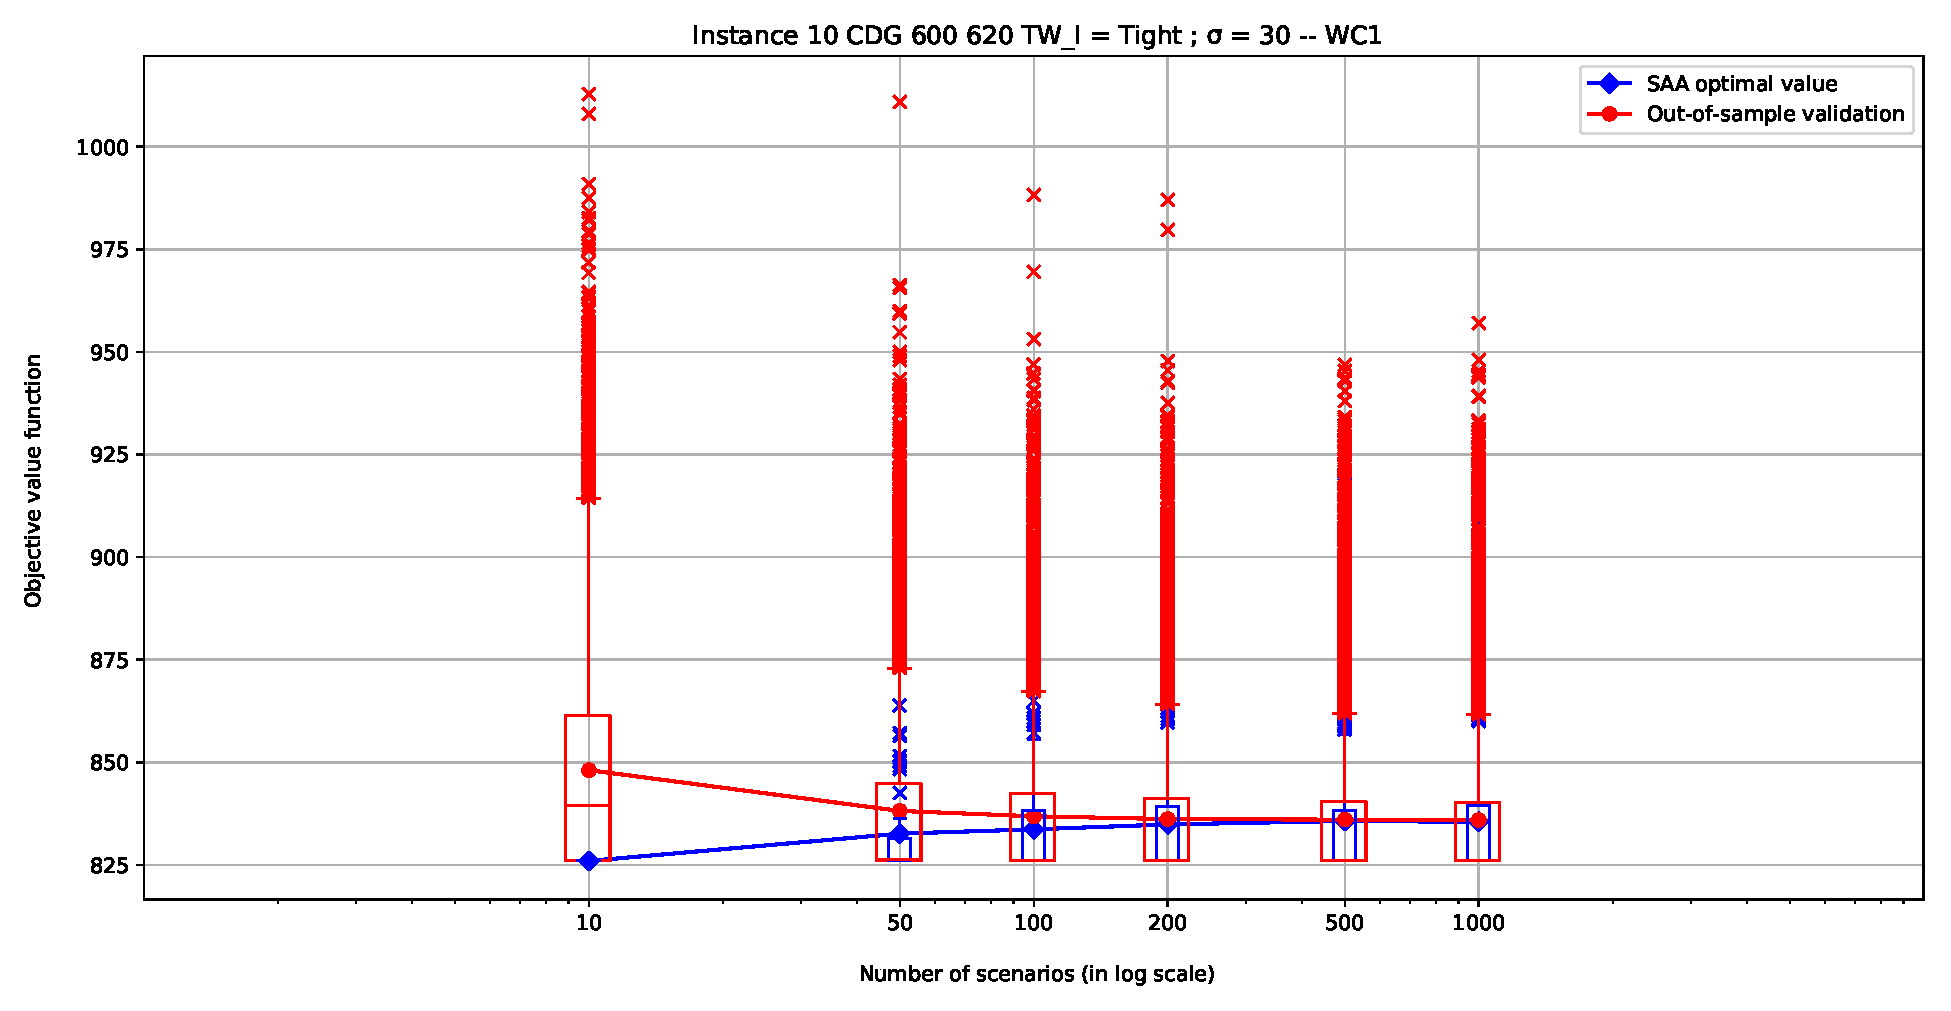
\includegraphics[width=\textwidth]{imgs/instance_landing.pdf}
\end{center}
\begin{small}
\textit{Ahmed Khassiba (2020), ``Two-stage stochastic programming for aircraft arrival scheduling under uncertainty'', Ph.D. thesis.}
\end{small}

\end{frame}

\begin{frame}
	\frametitle{SAA - Chance constraints}
	
	We consider the problem
	\begin{align*}
		\min_{x \in \mathcal{X}}\ & f(x) \\
		\mbox{s.t. } & P[G(x,\xi) \leq 0] \geq 1 - \alpha,
	\end{align*}
	where $G: \mathcal{R}^n \times \Xi \rightarrow \mathcal{R}^m$.
	
	This allows to consider separate and joint chanced constrained.
	
	We can reformulate this problem as
	\begin{align*}
		\min_{x \in \mathcal{X}}\ & f(x) \\
		\mbox{s.t. } & P[G(x,\xi) > 0] \leq \alpha,
	\end{align*}
	
	
	\mbox{}
	
	If $P[G(x,\xi) \leq 0]$ has no closed form, we can always approximate it by sample average approximation.
	
\end{frame}

\begin{frame}
	\frametitle{SAA}
	
	With the indicator function of $(0,\infty)$
	\[
	\mathcal{I}_{(0,\infty)} =
	\begin{cases}
		1 & \mbox{if } t > 0,\\
		0 & \mbox{if } t \leq 0,
	\end{cases}
	\]
	we can rewrite the chance constraint as
	\[
	p(x) = E\left[ \mathcal{I}_{(0,\infty)} \left( G(x, \xi) \right) \right] \leq \alpha.
	\]
	
	Let $\xi_1,\ldots,\xi_N$ be an i.i.d. sample of $N$ realizations of $\xi$.
	We approximate the chance constraint by
	\[
	\hat{p}_N = \frac{1}{N} \sum_{j = 1}^N \mathcal{I}_{(0,\infty)} \left( G(x, \xi_j) \right) \leq \gamma
	\]
	
\end{frame}

\begin{frame}
	\frametitle{SAA (cont'd)}
	
	$\hat{p}_N(x)$ is equal to the proportion of times that $G(x,\xi_j) > 0$.
	$\gamma$ is not necessarily equal to $\alpha$, especially when we want to enlarge the feasible of the approximate problem.
	
	\mbox{}
	
	The approximate problem is
	\begin{align*}
		\min_{x \in \mathcal{X}}\ & f(x) \\
		\mbox{s.t. } & \hat{p}_N(x) \leq \gamma.
	\end{align*}
	
\end{frame}

\begin{frame}
	\frametitle{Theory}
	
	For theoretical justifications, see
	\begin{quote}
		B.K. Pagnoncelli, S. Ahmed, and A. Shapiro, ``Sample Average Approximation Method for Chance
		Constrained Programming: Theory and Applications'', Journal of Optimization Theory and Applications 142 (2), pp. 399--416, 2009.
	\end{quote}
	
	\mbox{}
	
	Especially, under some regularity conditions, we have
	\[
	sup_{x \in C} |\hat{p}_N(x) - p(x)| \rightarrow 0,
	\]
	w.p.1, as $N \rightarrow \infty$.
	
\end{frame}

\begin{frame}
	\frametitle{Convergence}
	
	Assume that  there is an optimal solution $\overline{x}$ of the true problem such that for any $\epsilon > 0$ there is $x \in \mathcal{X}$ with $\| x - \overline{x} \| \leq \epsilon$ and $p(x) < \alpha$.
	
	\mbox{}
	
	\begin{theorem}
		Suppose $\gamma = \alpha$, $\mathcal{X}$ compact, and $f(x)$ continuous.
		Then $\hat{v}_N \rightarrow v^*$, where $\hat{v}_N$ and $v^*$ are the optimal values of the approximate and true problems, respectively, and $D(\hat{S}_N,S) \rightarrow 0$ almost surely as $N \rightarrow \infty$.
	\end{theorem}
	
\end{frame}

\begin{frame}
	\frametitle{Application: call centers}
	
	Joint work with Thuy Anh Ta, Tien Mai, Wyean Chan, and Pierre L'Ecuyer.
	The next slides are due Thuy Anh Ta.
	
	\mbox{}
	
	{\color{red}A call center}: an  office used for receiving or transmitting customers requests by {\color{red}telephone}.
	
	
	\begin{itemize}
		\item A {\color{blue}call} represents a customer and it is classified by {\color{blue}type} ($K$ types). 
		\item Customers are served by {\color{blue}agents}.
		\item Agents sharing a common set of tasks form a {\color{blue}group} of agents ($I$ groups).
		\item A day is divided into {\color{blue}periods} ($P$ periods).
		\item The work schedule of an agent is determined by her {\color{blue}shift} ($Q$ shift configurations).
	\end{itemize}
	
\end{frame}

\begin{frame}{Performance measure}
	\begin{itemize}
		\item{} {\color{blue}{Performance measures} (PM)} allow to assess the quality of service (QoS) and
		efficiency of a call center, e.g., Service level (SL) and average waiting time (AWT), abandonment ratio, occupancy ratio, etc.
		\item {\color{blue}Service level (SL)}: the percentage of calls that are answered in a defined waiting threshold.
		\item {\color{blue}Average waiting time (AWT)}: the average (or mean) time a customer waited to have a service.
		\item{} QoS can be defined in the long run (expectations), or over a given time period (random variable).
	\end{itemize}
\end{frame}

\begin{frame}{Staffing, Scheduling and Routing}
	\begin{itemize}
		\item{} The objective is to minimize the operating cost of a call center under a set of constraints on certain PMs (SL or AWT).
		\item{} Staffing: deciding the number of agents $y_{i,p}$ of each group for each period in a day.
		\item{} Scheduling:  determining how many agents $x_{i,q}$ to assign to a set of predefined shifts.
		\item{} Routing: determining which agents are allowed to handle the call, and how agents are chosen when several agents are free.
		
	\end{itemize}
	%		\begin{figure}
	%			\includegraphics[width=0.4\linewidth]{figures/planning.pdf}%
	%		\end{figure} 
\end{frame}

\begin{frame}{Modeling a call center}
	\begin{itemize}
		%		\item{} Different types of calls arrive at random and different groups of agents answer these calls
		\item{} The calls arrive according	to arbitrary stochastic processes that could be non-stationary (e.g. homogeneous Poisson process), and perhaps doubly stochastic (e.g. Poisson gamma process, the arrival rate is a random	variable of gamma distribution).
		\item{} Service times: exponential, log-normal distributions.
		%of calls are traditionally assumed as independent and identically distributed exponential random variables with a constant mean.
		\item{} Delay time,  patience time, etc.
		\item{} When number of skills is low: Arrivals are served in a first come first serve (FCFS) order and/or a longest idle server first rules. 
		\item{} Otherwise, {\color{blue}skills based routing} may be used to route calls to appropriate agents.
	\end{itemize}
\end{frame}

\begin{frame}{Staffing and scheduling with predictable arrival rates}
	\[
	g(y) = \frac{\mathbb{E}[\# \text{of served call that waited at most } \tau]}{\mathbb{E}[\# \text{ Total } \# \text{ of calls}]}
	\]
	\textbf{Scheduling problem}	
	\[
	\min {c}^T{x} = \sum_{i=1}^I\sum_{q=1}^Q c_{i,q}x_{i,q}
	\]
	subject to:
	\begin{equation} \tag{P1}
		\begin{aligned}
			{Ax} &\geq {y} \\
			g_{k,p}({y}) &\geq l_{k,p} ~\forall k,p, \\
			g_{p}({y}) &\geq l_{p} ~\forall p, \\
			g_{k}({y}) &\geq l_{k} ~\forall k, \\
			g(y) &\geq l,\\
			{x},{y}&\geq 0 \text{ and integer}  \text{.}\\
		\end{aligned}
	\end{equation}
\end{frame}

\begin{frame}{Staffing and scheduling with predictable arrival rates}
	\textbf{Staffing problem}	
	\[
	\min_y {c'}^T y = \sum_{i=1}^I\sum_{p=1}^P c'_{i,p}y_{i,p}
	\]
	subject to:
	\begin{equation} \tag{P2}
		\begin{aligned}
			g_{k,p}({y}) &\geq l_{k,p} ~\forall k,p, \\
			g_{p}({y}) &\geq l_{p} ~\forall p, \\
			g_{k}({y}) &\geq l_{k} ~\forall k, \\
			g(y) &\geq l,\\
			{y}&\geq 0 \text{ and integer}  \text{.}\\
		\end{aligned}
	\end{equation}
\end{frame}

\begin{frame}{Staffing and scheduling}
	
	SL $S(\tau, y)$ and AWT $W(y)$ are considered as r.v. in a given period.
	
	The chance-constrained scheduling problem for multiskill call centers is formulated as:
	\[
	\min {c}^T{x} = \sum_{i=1}^I \sum_{q=1}^Q c_{i,q}x_{i,q}
	\]
	subject to:
	\begin{equation} \tag{P3}
		\begin{aligned}
			{Ax} &\geq {y} \\
			\mathbb{P}[S_{k,p}(\tau_{k,p}, {y}) \geq s_{k,p}] &\geq r_{k,p} \text{\qquad{}}  \forall k,p \\
			\mathbb{P}[W_{k,p}(y) \leq w_{k,p}] &\geq  v_{k,p} \text{\qquad{}} \forall k,p\\
			{x}, {y} &\geq 0 \text{ and integer}. \\
		\end{aligned}
	\end{equation}
\end{frame}


\begin{frame}{Sample average approximate problem}
	\[
	\min {c}^T{x} = \sum_{i=1}^I \sum_{q=1}^Q c_{i,q}x_{i,q}
	\]
	subject to:
	\begin{equation} \tag{SAA} \label{s1}
		\begin{array}{ll}
			{Ax} &\geq {y} \\
			\displaystyle \frac{1}{N} \sum_{d=1}^N\mathbb{I}[\hat{S}_{N, k,p}^d(\tau_{k,p}, {y}) \geq s_{k,p}] &\geq r_{k,p} \text{\qquad{}}\forall k,p\\
			\displaystyle \frac{1}{N}\sum_{d=1}^N\mathbb{I}[\hat{W}_{N,k,p}^d({y}) \leq w_{k,p}]&\geq v_{k,p} \text{\qquad{}}\forall k,p\\
			{x}, {y} &\geq 0 \text{ and integer}  \text{ .}\\
		\end{array}
	\end{equation}
	Under some specific conditions, the optimal value and the set of optimal solutions of the SAA problem converge to those of the true problem  with probability one as $N$ approaches infinity. 
\end{frame}

\end{document}